\chapter{Methods}
\begin{enumerate}
    \item TODO: SQUASH SECTION BELOW INTO FEWER SECTIONS AND MAKE IT FLOW
    \item TODO: DETAIL
\end{enumerate}

\section{Sources of data}

Data is obtained in previous studies by A.\ Soylu, M.\ Zhou, and Ludo X\marginnote{What is Ludo's name? And ref to paper?} at the Medical Imaging center of the VUmc, Amsterdam.
\marginnote{Agreement?}
Human thigh and abdomen skin tissue were excised.
Pieces of these tissues were imaged with multiphoton microscopy and their stress-strain response curves were measured mechanically.
Data is acquired in batches from April 2021 until July 2022.
Development and testing data come from the same source.

Cadavers were eligible for thigh skin excision and abdomen skin is cut during plastic surgery.\marginnote{is this true?}
It is unknown if individuals received treatment relevant for this study.


\section{Data preparation}\label{sec:skin_data_prep}

\subsection{Preprocessing}

Depth stack images with a size of $\qty{1000}{px}\times\qty{1000}{px}$of all skin tissues were kindly provided by M.\ Zhou.
All stacks were separated into slices.

Images consist of three channels: third and second harmonic generation, and autofluorescence.
The SHG channel is chosen as it is assumed to only contain collagen information.

The SHG images are enhanced with contrast limited adaptive histogram equalization (CLAHE) \cite{Zuiderveld1994ContrastLA} using scikit-image \cite{scikit-image} to equalize importance of dark and bright regions.

The enhanced images are then transformed with a Yeo-Johnson transform such that the histogram of all images is as normal as possible.

The transformed images are standardized by subtracting the total mean and total standard deviation of the complete transformed image set, like
\begin{equation}
    X_\mathrm{out} = \frac{X_\mathrm{in} - \mu}{\sigma},
\end{equation}
where
\begin{equation}
    \mu = \frac{1}{N} \sum_i \sum_j \sum_k X_{i,j,k},
\end{equation}
and
\begin{equation}
    % \sigma = \sqrt{\frac{1}{N} \sum_{i,j,k} X_{i,j,k}^2 - \left(\frac{1}{N} \sum_{i,j,k} X_{i,j,k}\right)^2},
    \sigma = \sqrt{\frac{1}{N} \sum_i \sum_j \sum_k \left(X_{i,j,k} - \mu\right)^2},
\end{equation}
with $N$ the total number of pixels, $k$ an individual image and $i,j$ the pixel in the horizontal and vertical dimension, respectively.

The images are downsampled to $\qty{258}{px}\times \qty{258}{px}$ to fit into the neural network.

\subsubsection{Image selection}
SHG microscopy images from skin tissue suffer from optical phenomena.
The most evident problem is that imaging deeper into the tissue, photons are detected with less spatial accuracy thanks to scattering.
The deeper photons travel into tissue, the more possible paths photons can take to return to the detector.
Moreover, the chance of photons getting absorbed by the tissue increases with penetration depth.
Therefore, less photons get reflected from deeper tissue.

To counter these optical effects, inspired by \textcite{Koho2016} and \textcite{Blokker2022}, measures to quantify image quality can be obtained.
With this, images can be sorted to this measure and the top $k$ images with best quality can be used to train the network, thus excluding noise.

Candidates for this measure are Shannon entropy, kurtosis, and skew for reasons explained in \ref{subsec:imq}
These quality measures are calculated per image, such that the quality measure can be validated by observing manually.

\subsubsection{Image denoising}
Another optical disadvantage of multiphoton microscopy is the occurrence of noise.\marginnote{Look up sources of noise.}

Unfortunately, obtaining clearer images is hard.
Given the experimental setup as in (ref\marginnote{Actually refer to the paper describing the setup, which is written by whom?!}), one way to reduce noise in the image is to use more photons.
Either by averaging more images or increasing the amount of photons per image.
Increasing the amount of photons penetrating the tissue increase the risk of damaging the tissue.

Another way to deal with noisy images is to process the images.
Promising denoising neural networks have been developed.
The difficulty with this is that clean target data for supervised training is often not available in a biomedical setting.
To counteract this, Noise2Noise (N2N) \cite{Lehtinen2018} was developed.
Noise2Void N2V \cite{Krull2019}, a successor of N2N, does not rely on pairs of noisy images.
Instead it only needs one image and corrupts it to use as target and learns a mapping between the noisy image and the newly created noisy image.
This is useful if only one biomedical image is available.\marginnote{If denoised is used, move parts of this section to a theory section and refer to it here.}

The original N2V model produces a checkerboard pattern.
Noise2Void2 (N2V2) \cite{Hock2022} is an extension to N2V and reduces this artifact.\marginnote{Actually didn't do denoising, but if done, describe how here :)}

\subsection{Data augmentation}

To make the model more robust, data augmentation is applied.
Before the downsampling, the preprocessed images are cropped randomly from $\qty{1000}{px}\times \qty{1000}{px}$ to $\qty{700}{px}\times \qty{700}{px}$ preserving the aspect ratio.
The global brightness is adjusted randomly with $\pm \qty{30}{\percent}$.
The images are then randomly mirrored horizontally and vertically with a probability of \qty{50}{\percent}.

\section{Outcome}
The strain-stress response curves of individual skin tissue pieces were the outcome of interest.
The prediction is assessed by comparing it with measured strain-stress curves.\marginnote{Describe this comparison}
The measurement is done mechanically by an experimentalist.
The mechanical measurement itself is blind to clinical information.

\section{Predictors}\label{sec:skin_predictors}

% --------------------------------------------------
% SEARCHING FOR A SIMPLE SKIN STRAIN-STRESS MODEL
% --------------------------------------------------

\subsection{Searching for a simple skin strain-stress model}

Supervised learning requires targets for the model to train on.
Ideally, individual targets allow for physical interpretation and can together describe all the available data.

\subsubsection{Empirical strain-stress regions}
Although skin tissue has a complex nature, measurements to quantify skin stretch show similar features.
Measurements always show three domains: the toe, heel and leg domain (see fig.).
The toe region is at the very start of the curve.
This region is seems relatively flat as the fiber network consists of mostly unstretched fibers.
Therefore, the fibers cannot exert force as a reaction to external stretching force.
However, in the heel region where skin tissue is stretched more, fibers can exert more force.
When enough force is exerted on the tissue, fibers stretch maximally and fibers react with maximum force in the leg region.
This region is observed to be roughly linear.
Overstretching the tissue then breaks the fiber network, decreasing the possibility to exert force.

\subsubsection{Exponential}
Strain-stress curves can be also be visualized by showing the log derivative of stress with respect to strain against the log of strain (fig).
Typically, this figure has three regions.
The first region indicates a linear relationship between small forces and small strain.
Then, the derivative increases until it reaches a purely exponential part.
If skin stretching follows this kind of behaviour, a simple mathematical model can be derived.
Inspecting the figure, the linear part shows the ordinary differential equation
\begin{equation}
    \frac{\mathrm{d}\sigma}{\mathrm{d}\gamma} \propto \sigma,
\end{equation}
where $\gamma = \chi - 1$.
Solving for $\sigma$, we get
\begin{equation}
    \sigma \propto e^{\lambda\gamma},
\end{equation}
where $\lambda$ is some factor dictating the speed with which the exponential increases.
At no extension, i.\ e.\ $\gamma=0$, it can be assumed that there is no stress.
Therefore,
\begin{equation}
    \sigma \propto e^{\lambda\gamma} - 1.
\end{equation}
At small extensions, i.\ e.\ $\lambda\gamma \ll 1$, $e^{\lambda\gamma} \approx (1 + \lambda\gamma + \ldots)$ using a Taylor expansion.
So
\begin{equation}
    \sigma_{\lambda\gamma\ll 1} \propto 1 + \lambda\gamma + \ldots - 1 \approx G_0 \gamma,
\end{equation}
where $G_0$ is some linear coefficient at small extensions.
In this work, $\gamma = \chi - 1$, where $\chi$ is the stretch.
The full expression then becomes
\begin{equation}\label{eq:exp}
    \sigma = \frac{G_0}{\lambda}\left(e^{\lambda(\chi - 1)}-1\right).
\end{equation}

This model assumes that data follows the previously described curve where there is a small rise at small extensions and an indefinitely exponentially increasing stress for larger extensions.

The exponential model is fit to some stress-strain curves using OriginPro~\cite{OriginPro}.

\subsubsection{Principal component analysis}
In an earlier study (ref A.\ Soylu), principal component analysis (PCA) is used to reduce the dimensionality of the strain-stress data.
In summary, after PCA, every measurement $Y$ can be approximated by
\begin{equation}\label{eq:pca}
    Y \approx Y_\mathrm{PCA} = \mathbf{A} \mathbf{V} + \bar{Y},
\end{equation}
where $\mathbf{A}$ and $\mathbf{V}$ are matrices containing respectively the eigenvalues and -vectors of the the measurement data.
$\bar{Y}$ is the measurement mean.
Choosing the first $p$ principal components allows for dimensionality reduction.

Using PCA to create eigenvalues to weight the eigenvectors has some caveats.
First, the training and test sets must be treated separately.
The test set has to be projected on the space spanned by the first $p$ eigenvectors of the training set.
This may induce problems as the test set could contain information that does not come close to
Second, PCA depends on interpolation, i.\ e.\ every strain-stress curve must be formed by either a set of strain or stress values.
This reduces the domain of the data.

\subsubsection{Logistic curve}
The empirical observations where the force response of skin tissue changes states, suggests a logistic curve, which can be written as
\begin{equation}\label{eq:logistic_curve}
    \sigma = \frac{\sigma_\mathrm{max}}{1+e^{-E_\mathrm{max} (\gamma - \gamma_c)}},
\end{equation}
where $\sigma$ and $\gamma$ are the stress and engineering strain, $\sigma_\mathrm{max}$ is the maximum stress, $E_\mathrm{max}$ is the maximum Young's modulus and $\gamma_c$ the strain offset.
This equation assumes that there is a maximum force that the tissue can exert, in contrary to the theoretical approach above (ref).

Using the logistic curve as an alternative to PCA has two major advantages.
Every curve can be treated separately and measurements can contain data across arbitrary domains and with arbitrary intervals as no interpolation is necessary.

Strain-stress curves for all individuals were kindly provided by M.\ Zhou.
The curves only include datapoints where the skin extension is larger than zero and the force positive.

To every strain-stress curve, eq.~\ref{eq:logistic_curve} is fitted with Scipy \cite{2020SciPy-NMeth}.
The optimal parameters were be used for training the model.

BIAS\marginnote{Include density/thickness analysis of Mengyao and the gender/age analysis of myself}

The AI was trained on a with LDS smoothed target variable distribution.
The targets were weighted with the inverse square root, to limit the impact of LDS.

\section{Sample size}
The sample size is arrived at taking into account all previously included subjects (ref ludo, ref mengyao, ref alperen) and excluding abdomen data.
This amounts to a total of 1649 SHG images to train on.
For a detailed summary of the number of samples, see fig. (graph with nodes and edges explaining number of images/curves).

\section{Missing data}
Due to the limited amount of participants, individuals with unknown gender or age were included.

\section{Statistical analysis methods}

This section shows the methods obtain a trained model from stress-strain curves and images to use it for inference and interrogate it with XAI techniques.
The statistical methods are summarized in \cref{fig:skin_stat_methods}.

\begin{figure*}[p]
    \centering
    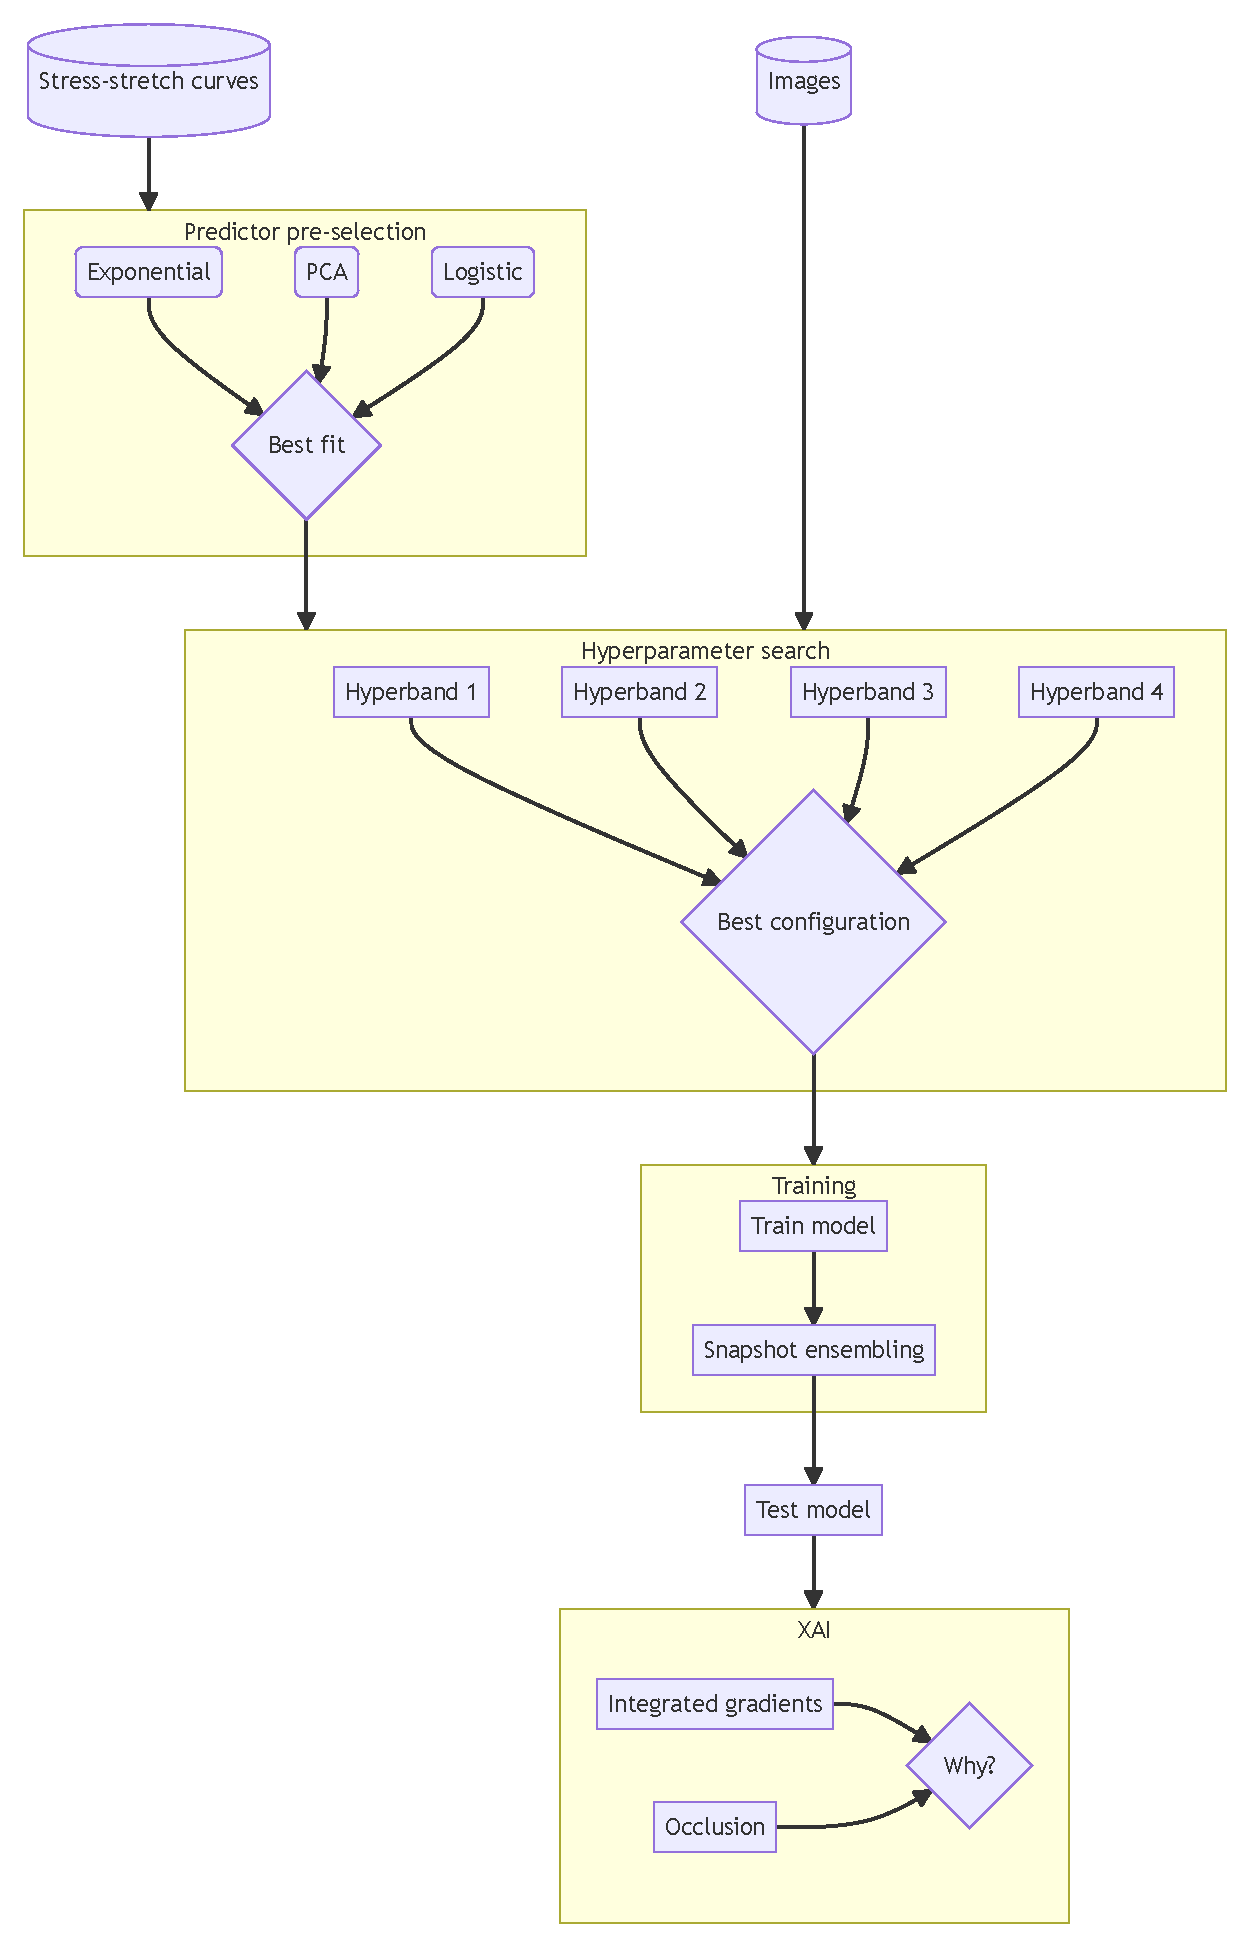
\includegraphics[height=\dimexpr\textheight-55.89pt\relax]{mermaid/skin_analysis.pdf}
    \caption[Flowchart of statistical analysis methods for \textsc{Skinstression}]{
        Flowchart of statistical analysis methods for \textsc{Skinstression}.
        Exponentials, principal component analysis (PCA) reconstructions, and logistic curves were fit to the stress-strain curves.
        The best-fitted model was used to create training targets.
        The targets and images were used as input for further training.
        The hyperparameter search was performed by four Hyperband studies and the best configuration was used for further training.
        After training, Snapshot Ensembling was used to build a final model.
        The final model is tested and interrogated using the XAI techniques integrated gradients and occlusion.
    }
    \label{fig:skin_stat_methods}
\end{figure*}

\subsection{Predictor pre-selection}
As discussed in \cref{sec:skin_predictors}, there are three predictor candidates.
These candidates are tested against the original strain-stress curves.

\subsubsection{Exponential and logistic curve}
The exponential and logistic models are fitted to all raw strain-stress curves.
The goodness of fit is determined by the coefficient of determination (\cref{subsec:coef_det}) and by eye.
A fit is considered good if it passes reasonably through all data points.
In particular, the exponential regime of the fit should describe the leg part of the curve.

\subsubsection{Principal component analysis}
PCA requires information on at least one axis to align between every curve.
The first step to achieve this is excluding all stretch values above the stretch of the maximum of the shortest curve.
\textcite{Soylu2022} did linear interpolation on the curves and restricted both stretch and stress to minim peak value.
PCA on two variables requires only one shared set of points.
Moreover, results of \citeauthor{Soylu2022} show knicks in the PCA reconstructions near the end of the curves, which could originate from a limited amount of datapoints or linear interpolation.
Therefore, in this study, a non-uniform, univariate, interpolating spline was fitted to all points and the stress was calculated from the spline at the stetch values of the curve with the lowest maximum stretch.
After PCA on the complete dataset, the explained variance per component was calculated and used as a method to find an appropriate number of principal components.
From these principal components, the curves where reconstructed using \cref{eq:pca}.
The goodness of fit is determined by the coefficient of determination (\cref{subsec:coef_det}) and by eye.
A fit is considered good if it passes reasonably through all data points and has few inflection points.

Only if PCA on the full dataset works reasonably well, it is possible to use PCA on a subset and use it to reconstruct another subset.
This would be useful if PCA was used to construct predictors, as using PCA results of the full dataset introduce information leakage from the test sets to the training set, because the components describe data from both subsets.
This is unlike Ref.~\cite{Soylu2022} where information leakage was not considered.\marginnote{Where to put PCA bias study?}

\subsection{Convolutional neural network}
The basis of the model originates from Liang \emph{et al.} \cite{Liang2017} and is adapted by Soylu \cite{Soylu2022}.
The model, a convolutional neural network, consists of five blocks.
The first block consists of a convolutional layer with a $\qty{3}{px}\times\qty{3}{px}$ kernel, taking in one channel and have 64 channels as output.
The output is then normalized per batch using BN (\cref{sec:bn}).
The normalized batch is passed through a ReLU (\cref{subsec:relu}) layer.
After activation, three $\qty{2}{px}\times\qty{2}{px}$ maxpool (\cref{subsec:maxpool}) layers are applied.
The next second block is like the first block, but with a $\qty{5}{px}\times\qty{5}{px}$ convolution kernel en just one maxpool layer.
The third block is like the second block, but with a $\qty{3}{px}\times\qty{3}{px}$ convolution kernel.
The fourth block is like the second and third block, but with a $\qty{6}{px}\times\qty{6}{px}$ and without a maxpool layer.

The fifth block flattens the input and consists of a two linear layers.
The first linear layer maps 64 nodes to $N_\mathrm{nodes}$ nodes.
After the first linear layer, BN and ReLU activation is applied.
The second linear layer maps $N_\mathrm{nodes}$ nodes to 3 nodes.
A linear activation function ensures the output is continuous and unaltered.
The model is shown in \cref{fig:model}

\begin{figure*}
    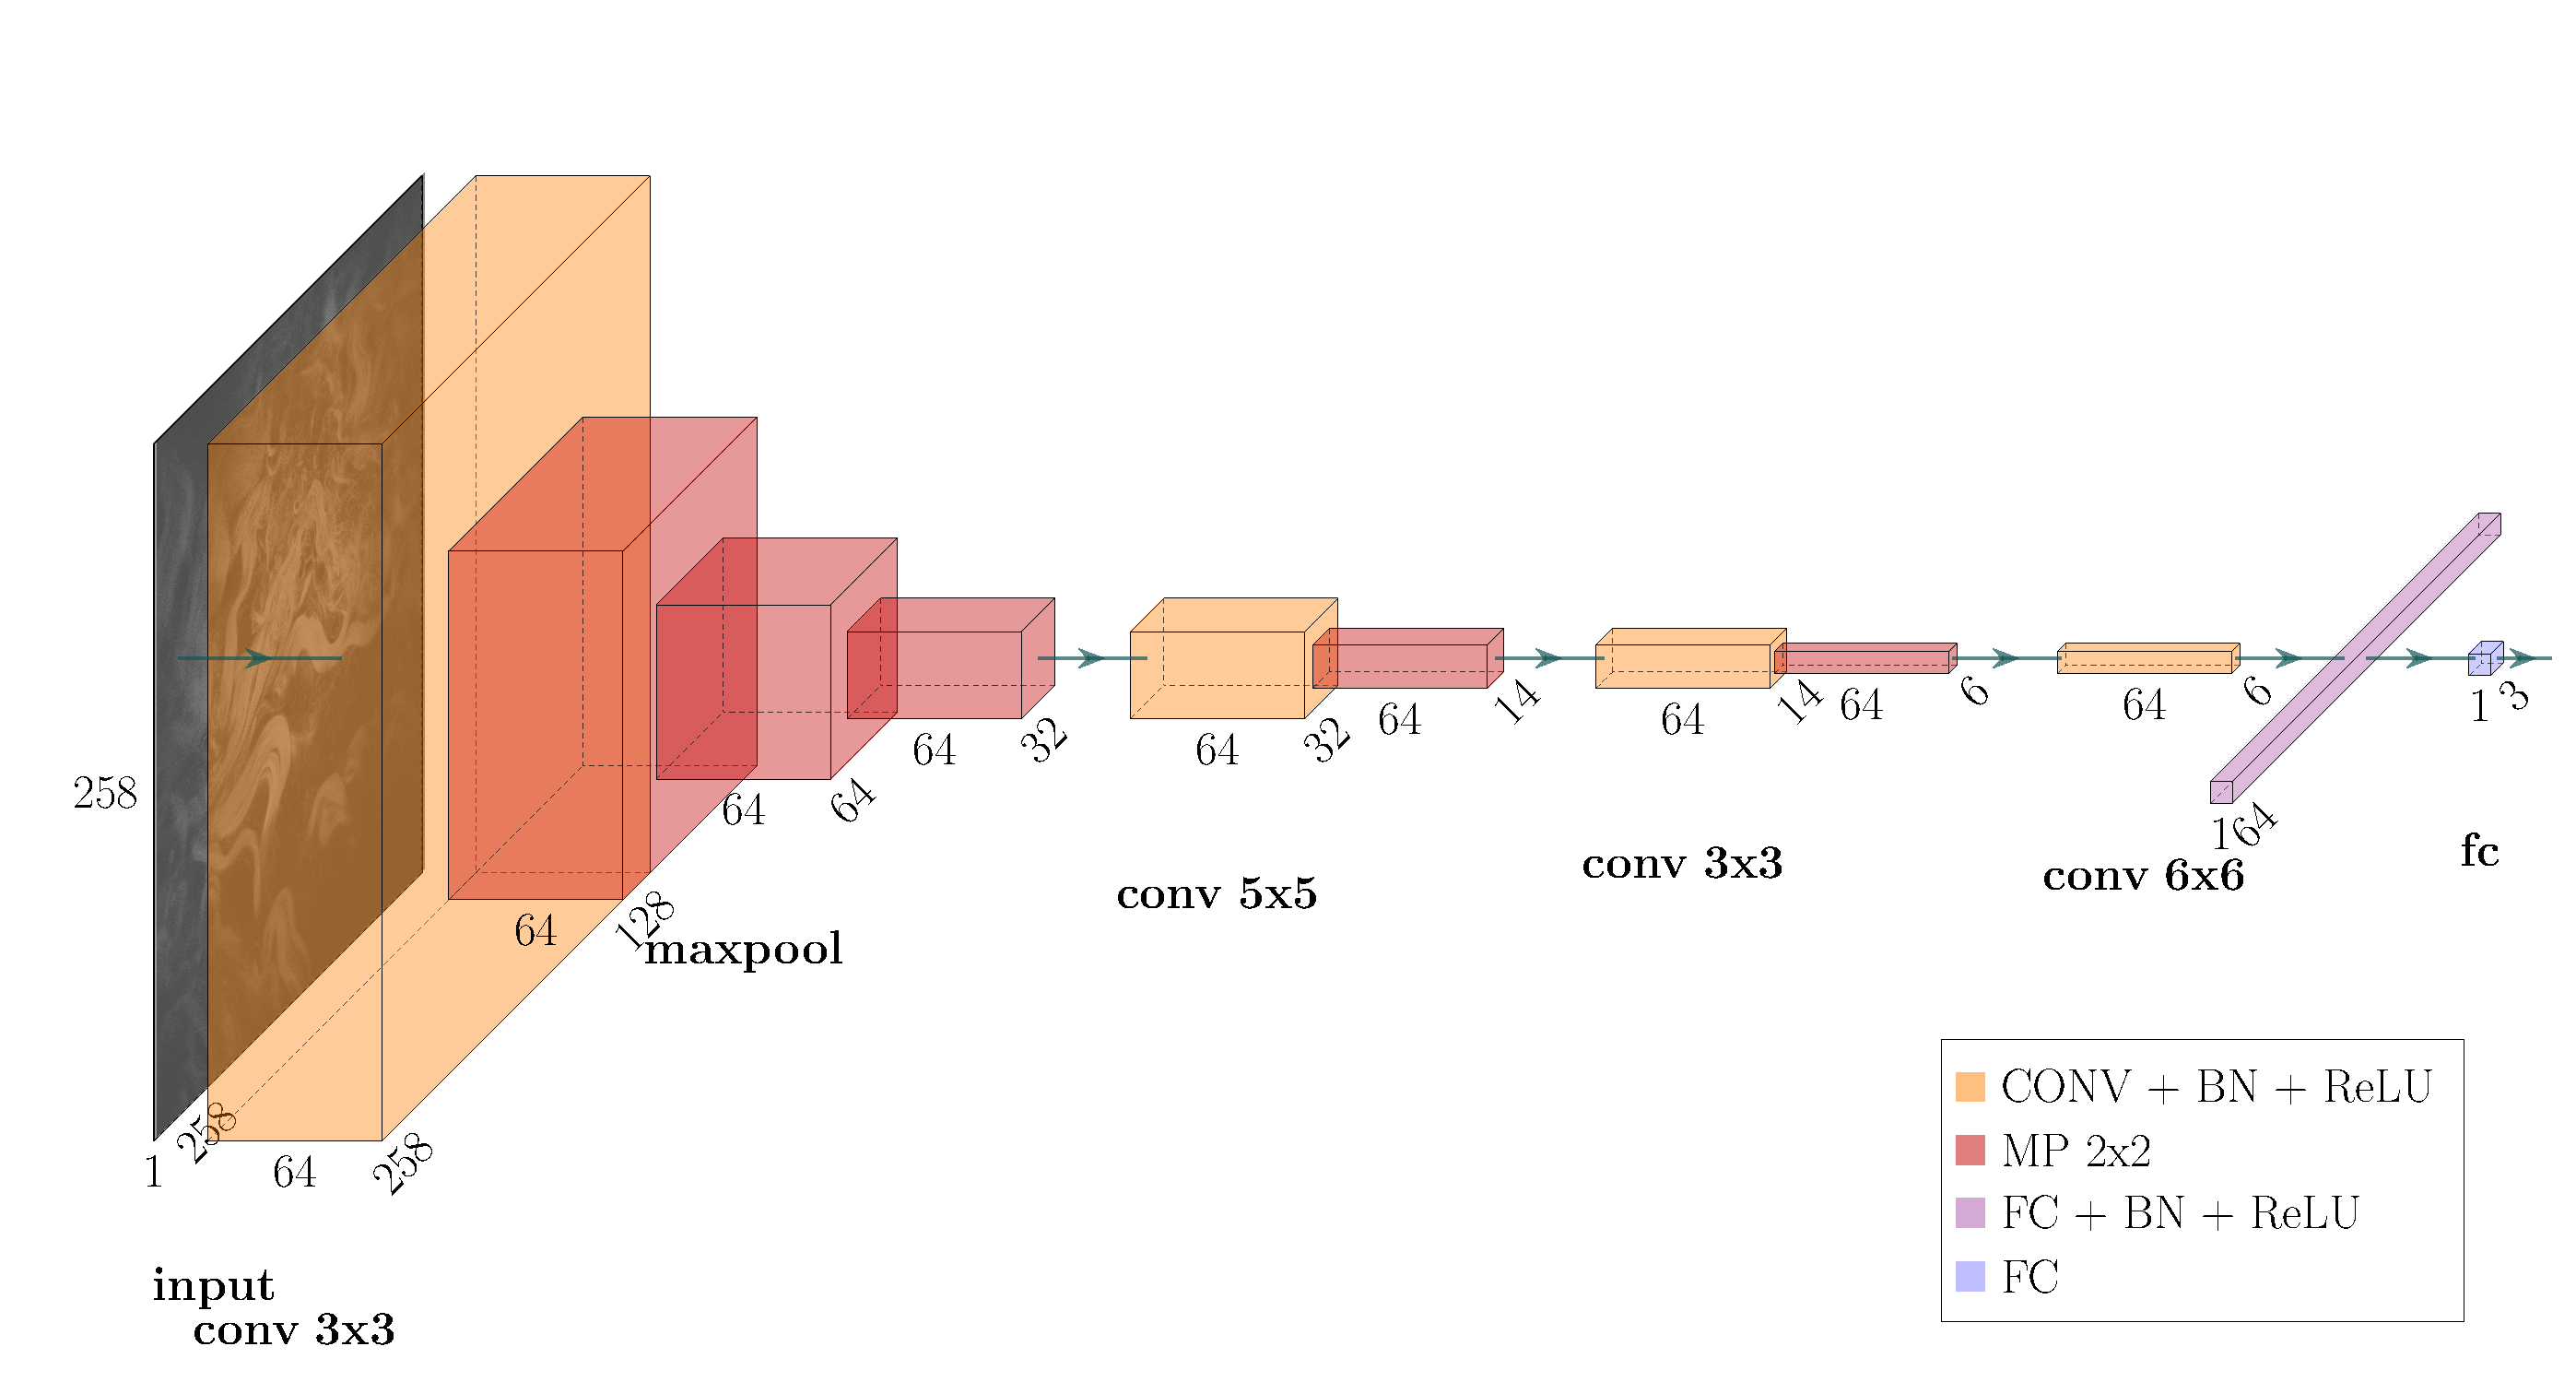
\includegraphics{skinstression/images/skinstression.pdf}
    % \input{PlotNeuralNet/examples/Skinstression/skinstression-new.tex}
    \caption[Network architecture]{
        The convolutional neural network consists of five blocks.
        The first four blocks contain convolution, maxpooling, and batch normalization layers.
        The last block contains a fully connected network.
        It requires an input of $\qty{258}{px}\times\qty{258}{px}$ to get a vector of length 3 as output.
    }
    \label{fig:model}
\end{figure*}

The dropout layers in \cite{Soylu2022} are replaced by BN layers, as the input is unnormalized and studies report better performance with BN.
Bias of all layers preceding BN layers have been set to zero.

The neural network weights are initialized according to the method described by \textcite{He2015a}, using a uniform transform.

\subsection{Hyperparameter optimization}
First, benchmark search 1 was done using Successive Halving with 100 trials.
See \cref{subsec:conf_skin} for a summary of configuration search space $\mathcal{C}$.
To allow trials to warmup, a minimum of 100 epochs were allowed.
To limit the trial duration, a maximum of 3000 epochs were allowed.
The number of trials were reduced with a reduction factor of $\eta=4$.
Trial parameters were sampled using the non-multivariate TPE algorithm.

The optimization was performed with the Adam optimizer ($\beta_1=0.9$, $\beta_2=0.999$), weighted focal MSE loss, and a cosine annealing with warm restarts learning rate scheduler.
Every trial used the complete dataset after data preparation (\cref{sec:skin_data_prep}).

The search uses a few data augmentations that are assumed to not alter the physical context of the image.
That is, force is exerted on the tissue in the horizontal direction in the image.
Therefore, flipping the image either vertically or horizontally is assumed to not change the stretch behaviour.
Both flipping operations occur with a probability of $0.5$.
Moreover, the images' intensity is randomly changed between x\% and x\%.\marginpar{By what fraction is the intensity changed?}

To possibly find a more optimal set of hyperparameters, two searches with the Hyperband algorithm with 300 trials was performed.
Trial parameters were sampled using the multivariate TPE algorithm.
The learning rate was warmed up linearly for the first 20 epochs.

% As shown in [ref results search 1], it seems that the network has difficulty with estimating $\gamma_c$, while $E_\mathrm{max}$ and $\sigma_\mathrm{max}$ seem to be easier estimated.
% As the original stress-strain curves do not have data in the plateau regime, $\sigma_\mathrm{max}$ was given less importance in search 2 and 3.
% This was achieved by weighting individual targets of the focal loss, such that
% \begin{equation}
%     FL = \frac{FL_{\sigma_\mathrm{max}} + FL_{E_\mathrm{max} + FL_{\gamma_c}}}{3}
% \end{equation}
% Therefore, in search 2 and 3, the goal was to give less importance to $$

Search 2 introduces random $700\times700$ cropping to further artificially increase the number of available images to train on.
% Also included is the ability to weight the loss per target variable (not to be confused with LDS), to penalize hard variables more than easy variables.
% The targets were weighted as $(\sigma_\mathrm{max},E_\mathrm{max},\gamma_c) = (0.8, 1, 1)$, to give less attention to the plateau.
Search 3 includes the Yeo-Johnson transformation to see how input normalization affects the training outcome.

For a summary of the hyperparameter searches, see \cref{tab:skin_studies}.

\begin{table}
    \caption[\textsc{Skinstression} hyperparameter search studies]{
        Summary of settings for hyperparameter searches performed.
        Hyperparameters are grouped by operation type (image preprocessing, image augmenting, target weighting) and in applied order.
        Every search is done with the search space described in \cref{tab:conf_skin}.
    }
    \label{tab:skin_studies}
    \begin{tabular}{lcccc}
        % \toprule
        % Search                         & 1      & 2      & 3      & 4      \\
        % \midrule
        % CLAHE                          & \cmark & \cmark & \cmark & \cmark \\
        % Yeo-Johnson transform          & \xmark & \xmark & \cmark & \xmark \\
        % \midrule
        % Random $700\times700$ cropping & \xmark & \cmark & \cmark & \cmark \\
        % Intensity jitter               & \cmark & \cmark & \cmark & \cmark \\
        % Random horizontal flip         & \cmark & \cmark & \cmark & \cmark \\
        % Random vertical flip           & \cmark & \cmark & \cmark & \cmark \\
        % Random sharpness               & \xmark & \xmark & \xmark & \cmark \\
        % Random gaussian blur           & \xmark & \xmark & \xmark & \cmark \\
        % Random rotation                & \xmark & \xmark & \xmark & \cmark \\
        % \midrule
        % Target variable weighting      & \xmark & \cmark & \cmark & \cmark \\
        % \bottomrule

        \toprule
        Search                         & 1      & 2      & 3      \\
        \midrule
        CLAHE                          & \cmark & \cmark & \cmark \\
        Yeo-Johnson transform          & \xmark & \xmark & \cmark \\
        \midrule
        Random $700\times700$ cropping & \xmark & \cmark & \cmark \\
        Intensity jitter               & \cmark & \cmark & \cmark \\
        Random horizontal flip         & \cmark & \cmark & \cmark \\
        Random vertical flip           & \cmark & \cmark & \cmark \\
        Random sharpness               & \xmark & \xmark & \xmark \\
        Random gaussian blur           & \xmark & \xmark & \xmark \\
        Random rotation                & \xmark & \xmark & \xmark \\
        % \midrule
        % Target variable weighting      & \xmark & \cmark & \cmark \\
        \midrule
        Search algorithm               & SH     & HB     & HB     \\
        Multivariate TPE               & \xmark & \cmark & \cmark \\
        trials                         & 100    & 300    & 300    \\
        learning rate warmup           & \xmark & \cmark & \cmark \\
        \bottomrule
    \end{tabular}
\end{table}

\subsection{Training}
Using the best configuration for hyperparameter optimization, a model is trained further for a total of 10000 epochs.
The learning rate scheduler was cosine annealing with warm restarts to allow for model ensembling later during inference (\cref{subsec:model_ensembling}).
The learning rate was warmed up linearly for the first 20 epochs.
To see the influence of image quality, the model is trained using an ordered set of images.
The images are ordered with maximum entropy first and the model is trained on all images and the top 5, 10, 15, and 20 images.

\subsection{Dataset}\label{subsec:skin_dataset}
The thigh dataset is randomly distributed into a training (\qty{64}{\percent}), validation (\qty{16}{\percent}), and test (\qty{20}{\percent}).
The distribution is stratified by person, meaning samples corresponding to the same person cannot live in two subsets simultaneously.
The AI learns from the training set.
Every iteration, it is validated against the validation set.
During inference, the AI is applied to the test set as external validation.

% \subsection{Model selection}
% MISSCHIEN MODEL ENSEMBLING EN VALIDATION SET GEBRUIKEN VOOR VINDEN VAN BESTE AANTAL MODELS?
% The last $N$\marginnote{How many again?} models are ensembled together

\section{Explainability}
To explain the model output, occlusion \cref{subsec:occlusion} is used.
Using the Captum Python library \cite{Kokhlikyan2020}, occlusion is done with $20\times 20$\unit{px} square patches moving with strides of 1.
All values in the patch have been replaced with 0.
